\def\deso{0}
\begin{name}
	{\tenchude}
	{\tendethi}
	{\tentruong}
	{\thoigian}
\end{name}
\TN
\Opensolutionfile{ans}[ans/2-PT-TNTHPT2025-De1-TN]

\begin{ex}%[2H2H1-2]
	\immini{
	Cho tứ diện $ABCD$. Gọi $M$, $N$ lần lượt là trung điểm của $BC$, $CD$. Gọi $G$ là trọng tâm của tam giác $BCD$.
	Khẳng định nào sau đây đúng?
	\choice
	{$\overrightarrow{G M}+\overrightarrow{G N}=\overrightarrow{0}$}
	{\True $\overrightarrow{G B}+\overrightarrow{G C}+\overrightarrow{G D}=\overrightarrow{0}$}
	{$\overrightarrow{G A}+\overrightarrow{G B}=\overrightarrow{0}$}
	{$\overrightarrow{G A}+\overrightarrow{G B}+\overrightarrow{G C}=\overrightarrow{0}$}
	}{
	\begin{tikzpicture}[scale=0.9, font=\footnotesize, line join=round, line cap=round, >=stealth]
		\path
		(2,2.5) coordinate (A)
		(0,0) coordinate (B)
		(1,-1.5) coordinate (C)
		(4,0) coordinate (D)
		($(B)!0.5!(C)$) coordinate (M)
		($(D)!0.5!(C)$) coordinate (N)
		($(B)!2/3!(N)$) coordinate (G)
		;
		\draw[->] (A)--(B);
		\draw[->] (A)--(D);
		\draw [dashed,->](A)--(G);
		\draw (B)--(C)--(D) (A)--(C);
		\draw [dashed](N)--(B)--(D)--(M);
		\foreach \x/\g in {A/90,B/135,C/-45,D/-90,M/200,N/-30,G/-80}
		\fill (\x) circle (1.1pt) ($(\x)+(\g:3mm)$) node{$\x$};
	\end{tikzpicture}
	}
	\loigiai{
	Vì $G$ là trọng tâm tam giác $BCD$ nên $\overrightarrow{G B}+\overrightarrow{G C}+\overrightarrow{G D}=\overrightarrow{0}$.
	}
\end{ex}

\begin{ex}%[1H4H3-2]
	Cho hình chóp tứ giác $S.ABCD$. Gọi $M$ và $N$ lần lượt là trung điểm của $SB$ và $SD$. Khẳng định nào sau đây đúng?
	\choice
	{$MN \parallel (SBC)$}
	{$MN \parallel (SAB)$}
	{$MN \parallel (SCD)$}
	{\True $MN \parallel (ABCD)$}
	\loigiai{
	\immini{
	Ta có $\heva{&MN\parallel BD\\&BD\subset (ABCD)\\&MN\not\subset (ABCD)}$ suy ra $MN \parallel (ABCD)$.
	}{
	\begin{tikzpicture}[scale=1, font=\footnotesize, line join=round, line cap=round, >=stealth]
		\def \a{2.5}
		\path
		(0,0) coordinate (A)
		(0:\a) coordinate (B)
		(230:0.6*\a) coordinate (D)
		($(B)+(D)$) coordinate (C)
		(85:0.9*\a) coordinate (S)
		($(S)!0.5!(B)$) coordinate (M)
		($(S)!0.5!(D)$) coordinate (N)
		;
		\draw (B)--(C)--(D)--(S)--(B)(S)--(C);
		\draw[dashed] (S)--(A)--(B)--(D)--(A)(M)--(N);
		\foreach \x/\g in {A/-90,B/0,C/-20,D/180,S/90,M/30,N/160}\fill[black] (\x) circle (1pt)+(\g:.3)node{$\x$};
	\end{tikzpicture}
	}
	}
\end{ex}

\begin{ex}%[1D5H2-3]
	Bác Minh thống kê lại thời gian sử dụng điện thoại của mình từ khi điện thoại được sạc đầy pin cho đến khi pin được sử dụng hết trong $30$ ngày ở biểu đồ sau
	\begin{center}
		\begin{tikzpicture}[scale=.75]
			\draw[color=gray,dash pattern=on 1pt off 1pt,xstep=1.0cm,ystep=1.0cm] (0,0) grid (12.2,7);
			\foreach \i in {0,2,...,12}
			\draw (0,1*\i/2)node[left]{\bf\footnotesize $\i$} (-0.1,1*\i/2)--(0.1,1*\i/2);
			\draw (0,-0.1)--(0,0.1);
			\draw (1.5,0)node[below]{\footnotesize $[12;14)$};
			\path[fill=cyan,draw=white] (1,0)rectangle(2,2);
			\draw (3.5,0)node[below]{\footnotesize $[14;16)$};
			\path[fill=cyan,draw=white] (3,0)rectangle(4,4);
			\draw (5.5,0)node[below]{\footnotesize $[16;18)$};
			\path[fill=cyan,draw=white] (5,0)rectangle(6,5);
			\draw (7.5,0)node[below]{\footnotesize $[18;20)$};
			\path[fill=cyan,draw=white] (7,0)rectangle(8,3);
			\draw (9.5,0)node[below]{\footnotesize $[20;22)$};
			\path[fill=cyan,draw=white] (9,0)rectangle(10,1);
			\draw[<->,>=latex] (0,7)  node[above]{Số ngày}|-(13,0) node[below]{Thời gian sử dụng (giờ)};
			\draw (6,8)node[above]{\bf Biểu đồ tần số theo thời gian sử dụng};
			\draw (1.5,2) node[above]{$4$} (3.5,4)node[above]{$8$} (5.5,5)node[above]{$10$} (7.5,3)node[above]{$6$} (9.5,1)node[above]{$2$};
		\end{tikzpicture}
	\end{center}
	Tứ phân vị thứ nhất của mẫu số liệu ghép nhóm trên là
	\choice
	{$13{,}125$}
	{$14{,}4375$}
	{\True $14{,}875$}
	{$13{,}5625$}
	\loigiai{
	Tứ phân vị thứ nhất của mẫu số liệu ghép nhóm thuộc nhóm $[14;16)$.\\
	Tứ phân vị thứ nhất của mẫu số liệu ghép nhóm trên là $$Q_1=14+\dfrac{\dfrac{30}{4}-4}{8} \cdot (16-14)=14{,}875.$$
	}
\end{ex}

\begin{ex}%[2H5N2-2]
	Trong không gian $ Oxyz$, vectơ nào sau đây là một vectơ chỉ phương của trục $Oz$?
	\choice
	{${\vec j}=\left(0;1;0\right)$}
	{\True $\vec k=\left(0;0;1\right)$}
	{${\vec i}=\left(1;0;0\right)$}
	{${\vec u}=\left(1;1;1\right)$}
	\loigiai{
	Vectơ chỉ phương của trục $Oz$ là $\vec k=\left(0;0;1\right)$.
	}
\end{ex}

\begin{ex}%[2D4N1-2]
	Cho $a$, $b \in \mathbb{R}$, $a \neq 0$. Hàm số $y = \ln|ax+b|$ là một nguyên hàm của hàm số
	\choice
	{$y = \dfrac{-a}{ax+b}$}
	{$y = \dfrac{1}{ax+b}$}
	{\True $y = \dfrac{a}{ax+b}$}
	{$y = -\dfrac{1}{ax+b}$}
	\loigiai{
	Ta có $y' = (\ln|ax+b|)'=\dfrac{a}{ax+b}$.
	}
\end{ex}

\begin{ex}%[1D2N2-3]
	Cho cấp số cộng $(u_n)$ với $u_1=5$ và công sai $d=3$. Giá trị của $u_2$ bằng
	\choice
	{$15$}
	{$2$}
	{$-2$}
	{\True $8$}
	\loigiai{
	Ta có $u_2=u_1+d=5+3=8$.
	}
\end{ex}

\begin{ex}%[1D1N5-3]
	Các nghiệm của phương trình $2\sin3x+\sqrt{2}=0$ là
	\choice
	{$x=\dfrac{\pi}{12}+k\dfrac{2\pi}{3}$ và $x=\dfrac{3\pi}{12}+k\dfrac{2\pi}{3}$ $(k\in\mathbb{Z})$}
	{$x=\dfrac{\pi}{12}+k\dfrac{2\pi}{3}$ và $x=-\dfrac{\pi}{12}+k\dfrac{2\pi}{3}$ $(k\in\mathbb{Z})$ }
	{\True $x=-\dfrac{\pi}{12}+k\dfrac{2\pi}{3}$ và $x=\dfrac{5\pi}{12}+k\dfrac{2\pi}{3}$ $(k\in\mathbb{Z})$}
	{$x=-\dfrac{\pi}{12}+k\dfrac{2\pi}{3}$ và $x=\dfrac{3\pi}{12}+k\dfrac{2\pi}{3}$ $(k\in\mathbb{Z})$}
	\loigiai{
	\begin{eqnarray*}
		& & 2\sin3x+\sqrt{2}=0\\
		&\Leftrightarrow& \sin 3x=-\dfrac{\sqrt{2}}{2} \\
		&\Leftrightarrow& \sin 3x=\sin\left(-\dfrac{\pi}{4} \right) \\
		&\Leftrightarrow& \hoac{&3x=-\dfrac{\pi}{4}+k2\pi\\&3x=\pi-\left( -\dfrac{\pi}{4}\right) +k2\pi}\\
		&\Leftrightarrow& \hoac{&x=-\dfrac{\pi}{12}+k\dfrac{2\pi}{3}\\&x=\dfrac{5\pi}{12}+k\dfrac{2\pi}{3}} (k\in \mathbb{Z}).
	\end{eqnarray*}
	}
\end{ex}

\begin{ex}%[2D4N3-1]
	Cho hàm số $y=f(x)$ xác định và liên tục trên đoạn $[a;b]$. Diện tích hình phẳng giới hạn bởi đồ thị hàm số $y=f(x)$, trục hoành và hai đường thẳng $x=a$, $x=b$ được tính theo công thức
	\choice
	{$S=-\displaystyle\int_{a}^{b}f(x)\mathrm{\,d}x$}
	{$S=\displaystyle\int_{a}^{b}f(x)\mathrm{\,d}x$}
	{\True $S=\displaystyle\int_{a}^{b}|f(x)|\mathrm{\,d}x$}
	{$S=\displaystyle\int_{b}^{a}|f(x)|\mathrm{\,d}x$}
	\loigiai{
	Công thức tính diện tích hình phẳng giới hạn bởi đồ thị hàm số $y=f(x)$, trục hoành và hai đường thẳng $x=a$, $x=b$ là $S=\displaystyle\int_{a}^{b}|f(x)|\mathrm{\,d}x$.
	}
\end{ex}

\begin{ex}%[2H5N1-3]
	Trong không gian $Oxyz$, viết phương trình mặt phẳng qua điểm $M\left(2;-3;4\right)$ và nhận $\overrightarrow{n}=(-2;4;1)$ làm một vectơ pháp tuyến.
	\choice
	{$2x-4y-z+10=0$}
	{$2x+4y+z-12=0$}
	{\True $2x-4y-z-12=0$}
	{$-2x+4y+z+11=0$}
	\loigiai{
	Phương trình mặt phẳng qua điểm $M\left(2;-3;4\right)$ và nhận $\overrightarrow{n}=(-2;4;1)$ làm một vectơ pháp tuyến là
	$$-2\left(x-2\right)+4\left(y+3\right)+1\left(z-4\right)=0\Leftrightarrow -2x+4y+z+12=0\Leftrightarrow 2x-4y-z-12=0.$$
	}
\end{ex}

\begin{ex}%[1D6N4-2]
	Tìm nghiệm của phương trình $\log_5 x=8$.
	\choice
	{$x=40$}
	{\True $x=390\,625$}
	{$x=13$}
	{$x=32\,768$}
	\loigiai{
	$\log_5 x=8 \Leftrightarrow x=5^8=390\,625$.
	}
\end{ex}

\begin{ex}%[2D1H4-1]
	Cho hàm số $y = f(x)$ liên tục trên $\mathbb{R}$ và có bảng xét dấu của đạo hàm như sau:
	\begin{center}
		
\begin{tikzpicture}
			\tkzTabInit[nocadre=false,lgt=1.2,espcl=3,deltacl=0.7]
			{$x$ /.6, $y'$ /.6}
			{$-\infty$,$-2$,$0$,$2$,$+\infty$}
			\tkzTabLine{,+,$0$,-,$0$,+,$0$,-,}
		\end{tikzpicture}
	\end{center}
	Số điểm cực đại của hàm số là
	\choice
	{$3$}
	{\True $2$}
	{$0$}
	{$1$}
	\loigiai{
	Từ bảng xét dấu, ta thấy hàm số có hai điểm cực đại là $x = -2$ và $x = 2$.
	}
\end{ex}

\begin{ex}%[1H8H7-2]
	Cho khối chóp $S.ABC$ có $SA$, $AB$, $AC$ đôi một vuông góc. Biết $SA = 3a$, $AB = 4a$, $AC = 2a$. Thể tích của khối chóp đã cho là
	\choice
	{$V = 2a^3$}
	{$V = 24a^3$}
	{$V = 6a^3$}
	{\True $V = 4a^3$}
	\loigiai{
	\immini{
	Ta có $V = \dfrac{1}{3} S \cdot h= \dfrac{1}{6} \cdot SA \cdot AB \cdot AC = \dfrac{1}{6} \cdot 3a \cdot 4a \cdot 2a = 4a^3$.}{
	\begin{tikzpicture} [>=stealth,line join=round,line cap=round,font=\footnotesize,scale=0.7]
		\path
		(0,0) coordinate (A)
		(5,0) coordinate (B)
		(2,-2) coordinate (C)
		(0,3) coordinate (S);
		\draw (S)--(B)--(C)--(S)--(A)--(C);
		\draw[dashed] (A)--(B);
		\foreach \x/\y in {A/180, B/0, C/-90, S/90}
		\draw[fill=black] (\x) circle (1pt) + (\y:0.3cm) node{$\x$};
		\path
		pic[draw,angle radius=5pt]{right angle= B--A--S}
		pic[draw,angle radius=5pt]{right angle= B--A--C};
	\end{tikzpicture}
	}
	}
\end{ex}

\Closesolutionfile{ans}
% \indapan{6}{ans/2-PT-TNTHPT2025-De1-TN}
\cauds
\Opensolutionfile{ans}[ans/2-PT-TNTHPT2025-De1-DS]

\begin{ex}%[Đề phát triển 01 - 2025]%[Duong Xuan Loi]%[2D1H3-1]
	Cho hàm số $h(x)=\dfrac{x^2-3x+3}{x-2}$.
	\choiceTF
	{\True Hàm số đã cho có đạo hàm là $h'(x)=\dfrac{x^2-4x+3}{(x-2)^2}$}
	{Phương trình $h'(x)=0$ có tập nghiệm là $S=\{1\}$}
	{$h(3)=1$}
	{Giá trị lớn nhất của hàm số $h(x)$ trên đoạn $[0; 1]$ bằng $3$}
	\loigiai{
	Hàm số $h(x)$ xác định và liên tục trên $\mathbb{R} \setminus \{2\}$.
	\begin{itemchoice}
		\itemch Ta có $h'(x)=\dfrac{(2x-3)(x-2)-(x^2-3x+3)(1)}{(x-2)^2}
		= \dfrac{x^2-4x+3}{(x-2)^2}$.
		\itemch Phương trình $h'(x)=0 \Leftrightarrow x^2-4x+3=0\Leftrightarrow \hoac{& x=1 \\ & x=3.}$\\
		Vậy tập nghiệm là $S=\{1; 3\}$.
		\itemch Ta có $h(3) = 3$.
		\itemch Xét hàm số $h(x)$ trên đoạn $[0; 1]$.\\
		Ta có $h'(x)=\dfrac{x^2-4x+3}{(x-2)^2}$.\\
		$h'(x)=0 \Leftrightarrow \hoac{& x=1\in[0;1] \\ & x=3\notin[0;1].}$
		\begin{center}
			
\begin{tikzpicture}
				\tkzTabInit[nocadre=false,lgt=1.2,espcl=3.5,deltacl=0.6]
				{$x$ /0.6, $h'(x)$ /0.6, $h(x)$ /2.1}
				{$0$,$1$}
				\tkzTabLine{,+,}
				\tkzTabVar{ -/$-1{,}5$,+/$-1$}
			\end{tikzpicture}
		\end{center}
		Vậy giá trị lớn nhất của hàm số $h(x)$ trên đoạn $[-0;1]$ bằng $-1$.
	\end{itemchoice}}
\end{ex}

\begin{ex}%[Đề phát triển 01 - 2025]%[Duong Xuan Loi]%[2D1V5-8]
	\immini{Trong một thí nghiệm xử lý nước thải tại phòng thí nghiệm, người ta quan sát sự thay đổi nồng độ một chất ô nhiễm (đơn vị: NTU – chỉ số biểu thị mức độ ô nhiễm, giá trị càng cao thì mức độ ô nhiễm càng lớn) trong bể nước theo thời gian $t$ (tính bằng giờ) kể từ khi bắt đầu thí nghiệm. Khi bắt đầu, một lượng hóa chất được đưa vào bể. Nhờ quá trình phản ứng, hấp thụ và tự phân hủy sinh học, mức độ ô nhiễm thay đổi theo thời gian và được mô phỏng xấp xỉ bằng công thức $y(t) = 5 - \dfrac{15t}{9t^2 + 1}$, với $t \geq 0$.
	(Đồ thị hình bên biểu diễn mức độ ô nhiễm của nước theo thời gian).
	}{
	\begin{tikzpicture}[>=stealth,x=1cm,y=0.3cm,scale=1.4,font=\footnotesize,line join=round, line cap=round]
		\draw[->] (-0.5,0) -- (4,0) node[below] {$t$};
		\draw[->] (0,-1) -- (0,6) node[left] {$y$};
		\filldraw (0,0) circle (1pt)node[below left]{$O$};
		\draw[domain=0:4,samples=200,black] plot (\x,{5-(15*(\x))/(9*(\x)^2+1)});
		\draw[dashed] (0,5) node [left] {$5$}--(4,5);
		\foreach \x/\g in {1/-90,2/-90,3/-90}
		\draw[thin] (\x,2pt)--(\x,-2pt) + (\g:3mm) node {$\x$};
	\end{tikzpicture}
	}
	\choiceTF
	{Sau thời điểm độ ô nhiễm đạt mức thấp nhất, nước đã đạt trạng thái sạch ổn định}
	{\True Trong toàn bộ quá trình theo dõi, nồng độ ô nhiễm không vượt quá $5 \, \mathrm{NTU}$}
	{\True Sau $1$ giờ kể từ khi thí nghiệm bắt đầu, nồng độ ô nhiễm trong nước là $3{,}5 \, \mathrm{NTU}$}
	{\True Nồng độ ô nhiễm đạt mức thấp nhất tại thời điểm $t = \dfrac{1}{3}$}
	\loigiai{
	\begin{itemchoice}
		\itemch
		Đồ thị cho thấy nồng độ ô nhiễm đạt mức thấp nhất tại $t = t_0<1$ giờ, nhưng sau đó lại tăng dần về giá trị $5 \, \mathrm{NTU}$. Do đó, nước chưa đạt trạng thái ổn định.
		\itemch
		Từ công thức $y(t) = 5 - \dfrac{15t}{9t^2 + 1}$, ta thấy
		$$
		\dfrac{15t}{9t^2 + 1} > 0 \  \forall t > 0  \Rightarrow  y(t) < 5 \  \forall t > 0 .
		$$
		Khi $t = 0$, $y(0) = 5$. Vậy nồng độ ô nhiễm luôn nhỏ hơn hoặc bằng $5 \, \mathrm{NTU}$.
		\itemch Ta có $y(1) = 5 - \dfrac{15 \cdot 1}{9 \cdot 1^2 + 1} = 5 - \dfrac{15}{10} = 5 - 1{,}5 = 3{,}5$ NTU.\\
		Do đó sau $1$ giờ kể từ khi thí nghiệm bắt đầu, nồng độ ô nhiễm trong nước là $3{,}5$ NTU.
		\itemch Ta có
		$y'(t) =\dfrac{135t^2-15}{(9t^2 + 1)^2}$.\\
		Suy ra $y'(t) = 0\Rightarrow 15 - 135t^2 = 0\Rightarrow t^2 = \dfrac{1}{9} \Rightarrow t = \dfrac{1}{3}$.\\
		Bảng biến thiên
		\begin{center}
			
\begin{tikzpicture}
				\tkzTabInit[nocadre=false,lgt=1.2,espcl=2.5,deltacl=0.6]
				{$t$/0.9,$y'(t)$/0.6,$y(t)$/1.6}
				{$0$,$\tfrac13$,$+\infty$}
				\tkzTabLine{,-,0,+,}
				\tkzTabVar{+/,-/,+/}
			\end{tikzpicture}
		\end{center}
		Vậy nồng độ ô nhiễm đạt mức thấp nhất tại thời điểm $t = \dfrac{1}{3}$.
	\end{itemchoice}
	}
\end{ex}

\begin{ex}%[Đề phát triển 01 - 2025]%[Duong Xuan Loi]%[2H5V1-7]
	Một bể cá hình hộp chữ nhật $ABCD.EFGH$ với $AB=3$ dm, $AD=4$ dm, và cạnh bên bằng $5$ dm. Chọn hệ trục $Oxyz$ trong không gian có gốc tọa độ $O$ trùng với $A$, tia $Ox$ chứa điểm $B$, tia $Oy$ chứa điểm $D$ và tia $Oz$ chứa điểm $E$.
	\begin{center}
		\begin{tikzpicture}[scale=0.7,font=\footnotesize,line join=round,line cap=round,>=stealth]
			\path
			(0,0) coordinate (A)
			(4,0) coordinate (B)
			(6,-2.5) coordinate (D)
			($(B)+(D)-(A)$) coordinate (C)
			($(A)+(90:3.5)$) coordinate (E)
			($(B)-(A)+(E)$) coordinate (F)
			($(C)-(A)+(E)$) coordinate (G)
			($(D)-(A)+(E)$) coordinate (H)
			($(A)!0.5!(F)$) coordinate (M)
			;
			\draw (E)--(A)--(D)--(C)--(G)--(F)--cycle (E)--(H)--(G) (H)--(D);
			\draw[dashed] (C)--(B)--(A)--(F)--(B);
			\foreach \p/\q in {A/160,B/45,C/-45,D/-90,E/90,F/90,G/30,H/50,M/140}
			\fill[black] (\p)node[shift={(\q:3mm)}]{$\p$} circle (1.0pt);
		\end{tikzpicture}
	\end{center}
	\choiceTF
	{\True Điểm $G(3;4;5)$}
	{$\overrightarrow{AF}\cdot\overrightarrow{EH}=1$}
	{$\tan \left((AFD),(BDC)\right)=\dfrac{5}{2}$}
	{\True Một chú cá con bơi theo những đoạn thẳng từ điểm $G$ đến chạm mặt đáy của bể, rồi từ điểm đó bơi đến vị trí điểm $M$ là trung điểm của $AF$. Để đường đi ngắn nhất thì chú cá bơi đến điểm dưới đáy bể cách $AB$ và $BC$ những đoạn bằng $a$ và $b$. Khi đó $T=9a^2+b=17$}
	\loigiai{
	\begin{itemchoice}
		\itemch
		Điểm $G(3;4;5)$.
		\itemch
		Do $ABCD.EFGH$ là hình hộp chữ nhật nên $EH\perp (ABFE)\Rightarrow EH\perp AF\Leftrightarrow\overrightarrow{AF}\cdot\overrightarrow{EH}=0$.
		\itemch
		Ta có $\heva{&(AFD)\cap (BDC)=AD\\&AF\perp AD,AF\subset (AFD)\\&AB\perp AD,AD\subset (BDC)}\Rightarrow \left((AFD),(BDC)\right)=(AF,AB)=\widehat{FAB}$. \\
		Mà $\tan\widehat{FAB}=\dfrac{FB}{AB}=\dfrac{5}{3}$ nên $\tan \left((AFD),(BDC)\right)=\dfrac{5}{3}$.
		\itemch  Gọi $Q$ là điểm cá bơi chạm đáy bể.\\
		$G(3;4;5), F(3;0;5),A(0;0;0)\Rightarrow M\left(\dfrac{3}{2};0;\dfrac{5}{2}\right)$.\\
		Gọi $R$ là điểm đối xứng của $M$ qua $(Oxy)$, khi đó $R\left(\dfrac{3}{2};0;-\dfrac{5}{2}\right)$.\\
		Với mọi $Q\in (Oxy)$ ta có $QM+QG=QR+QG\geq RG$.\\
		Do đó $(QM+QG)$ nhỏ nhất bằng $RG$ khi $Q$ là giao điểm của $RG$ với $(Oxy)$.\\
		$Q\in (Oxy)\Rightarrow Q(x;y;0)$, suy ra $\overrightarrow{GQ}=(x-3;y-4;-5)$, $\overrightarrow{GR}=\left(-\dfrac{3}{2};-4;-\dfrac{15}{2}\right)$.\\
		$Q$ thuộc đường thẳng $RG$ nên $\overrightarrow{GQ}$, $\overrightarrow{GR}$ cùng phương nên $\dfrac{x-3}{-\dfrac{3}{2}}=\dfrac{y-4}{-4}=\dfrac{-5}{-\dfrac{15}{2}}\Rightarrow x=2,y=\dfrac{4}{3}$.\\
		Vậy $Q\left(2;\dfrac{4}{3};0\right)\Rightarrow a=\dfrac{4}{3},b=3-2=1$ do đó $T=9a^2+b=17$.
	\end{itemchoice}}
\end{ex}

\begin{ex}%[Đề phát triển 01 - 2025]%[Duong Xuan Loi]%[2D6H1-3]
	Một công ty tham gia đấu thầu hai dự án. Khả năng thắng thầu các dự án lần lượt là $0{,}4$ và $0{,}5$. Khả năng thắng thầu cả hai dự án là $0{,}3$. Gọi $A$, $B$ lần lượt là biến cố thắng thầu dự án $1$ và dự án $2$.
	\choiceTF
	{Hai biến cố $A$ và $B$ độc lập}
	{\True Giả sử công ty thắng thầu dự án $1$, thì xác suất công ty thắng thầu dự án $2$ là $0{,}75$}
	{Giả sử công ty không thắng thầu dự án $1$, thì xác suất công ty thắng thầu dự án $2$ là $\dfrac{2}{3}$}
	{\True Xác suất công ty thắng thầu đúng $1$ dự án là $0{,}3$}
	\loigiai{
	\begin{itemchoice}
		\itemch
		Ta có $\mathrm{P}(A)\cdot\mathrm{P}(B)=0{,}4\cdot 0{,}5=0{,}2\neq 0{,}3=\mathrm{P}(AB)$.
		\itemch
		Xác suất để công ty thắng thấu dự án 2 khi đã biết thắng dự án $1$ là $\mathrm{P}(B|A)$.\\
		$\mathrm{P}(B|A)=\dfrac{\mathrm{P}(AB)}{\mathrm{P}(A)}=\dfrac{0{,}3}{0{,}4}=0{,}75$.
		\itemch
		Xác suất để công ty thắng thấu dự án 2 khi đã biết không thắng dự án 1 là $\mathrm{P}\left(B|\overline{A}\right)=\dfrac{\mathrm{P}\left(\overline{A}B\right)}{\mathrm{P}\left(\overline{A}\right)}$.\\
		Vì hai biến cố $\overline{A}B$ và $AB$ xung khắc nhau và $\overline{A}B\cup AB=B$ nên theo tính chất của xác suất ta có $$\mathrm{P}\left(B|\overline{A}\right)=\dfrac{\mathrm{P}\left(\overline{A}B\right)}{\mathrm{P}\left(\overline{A}\right)}
		=\dfrac{\mathrm{P}(B)-\mathrm{P}(AB)}{1-\mathrm{P}(A)}=\dfrac{0{,}5-0{,}3}{1-0{,}4}=\dfrac{1}{3}.$$
		\itemch
		Xác suất để công ty thắng thầu đúng $1$ dự án là $\mathrm{P}(C)$.\\
		$\mathrm{P}(C)=\mathrm{P}\left(A\cap\overline{B}\right)+\mathrm{P}\left(\overline{A}\cap B\right)=\mathrm{P}(A)-\mathrm{P}(A\cap B)+\mathrm{P}(B)-\mathrm{P}(A\cap B)=0{,}3$.
	\end{itemchoice}}
\end{ex}
\Closesolutionfile{ans}
% \indapan{2}{ans/2-PT-TNTHPT2025-De1-DS}

\caukq
\Opensolutionfile{ans}[ans/2-PT-TNTHPT2025-De1-KQ]

\begin{ex}%[1D2C2-5]
	\immini[thm]{Bạn Việt tham gia cuộc thi giải mật thư. Theo quy tắc của cuộc thi, người chơi cần chọn ra sáu số từ tập $S=\{25;26;27;28;29;30;31;32;33\}$ và xếp mỗi số vào đúng một vị trí trong sáu vị trí A, B, C, M, N, P như hình vẽ bên sao cho mỗi vị trí chỉ được xếp một số. Mật thư sẽ được giải nếu các bộ ba số xuất hiện ở những bộ ba vị trí (A, M, B); (B, N, C); (C, P, A) tạo thành các cấp số cộng theo thứ tự đó. Bạn Việt chọn ngẫu nhiên sáu số trong tập $S$ và xếp ngẫu nhiên vào các vị trí được yêu cầu. Gọi xác suất để bạn Việt giải được mật thư ở lần chọn và xếp đó là $a$. Giá trị của $\dfrac{22a + 3}{a}$ bằng bao nhiêu?
	\shortans{3802}
	}{\begin{tikzpicture}[scale=0.9, font=\bfseries, line join=round, line cap=round, >=stealth]
		\coordinate (A) at (0,4);
		\coordinate (B) at (-2,0);
		\coordinate (C) at (2,0);
		\coordinate (M) at ($(A)!0.5!(B)$);
		\coordinate (P) at ($(A)!0.5!(C)$);
		\coordinate (N) at ($(B)!0.5!(C)$);
		\draw (A)--(M)--(B)--(N)--(C)--(P)-- cycle;
		\foreach \diem/\nhan in {A/A, B/B, C/C, M/M, P/P, N/N}
		\node[draw, circle, minimum size=1cm, inner sep=0pt, fill=white] at (\diem) {\nhan};
	\end{tikzpicture}
	}
	\loigiai{Tập $S$ có $5$ số lẻ $\{25;27;29;31;33\}$ và $4$ số chẵn $\{26;28;30;32\}$.\\
	Số cách chọn $6$ số trong $9$ đã cho và sắp xếp là $n(\Omega)=\mathrm{A}_9^6=60480$.\\
	Gọi $A$ là biến cố ``chọn ngẫu nhiên sáu số trong tập $S$ và xếp ngẫu nhiên vào các vị trí theo yêu cầu''.\\
	Theo giả thiết, điều kiện ba bộ số tạo thành cấp số cộng nên ta có
	$$\heva{&A+B=2M \\& B+C=2N \\& C+A=2P.}$$
	Suy ra A, B, C cùng chẵn hoặc cùng lẻ và không lập thành một cấp số cộng.\\
	(Giả sử A, B, C theo thứ tự lập thành cấp số cộng thì $A+C=2B$, suy ra $2B=2P\Rightarrow B=P$, vô lí).\\
	\begin{itemize}
		\item \textbf{Trường hợp 1}: A, B, C cùng lẻ.\\
		Chọn $3$ số cùng lẻ có $\mathrm{C}_5^3$ cách, loại $4$ bộ (25;27;29), (27;29;31), (29;31;33), (25;29;33) (vì chúng lập thành cấp số cộng).\\
		Khi đó, có $\mathrm{C}_5^3-4=6$ (cách).\\
		Hoán vị bộ A, B, C có $3!$ cách xếp.\\
		Suy ra, trường hợp 1 này có $6\cdot 3!=36$ (cách xếp).
		\item \textbf{Trường hợp 2}: A, B, C cùng chẵn.\\
		Chọn $3$ số cùng chẵn có $\mathrm{C}_4^3$ cách, loại $2$ bộ (26;28;30), (28;30;32) (vì chúng lập thành cấp số cộng).\\
		Khi đó, có $\mathrm{C}_4^3-2=2$ (cách).\\
		Hoán vị bộ A, B, C có $3!$ cách xếp.\\
		Suy ra, trường hợp 2 này có $2\cdot 3!=12$ (cách xếp).
	\end{itemize}
	Từ hai trường hợp trên, ta có $n(A)=36+12=48$.\\
	Xác suất của biến cố $A$: $\mathrm{P}(A)=\dfrac{n(A)}{n(\Omega)}=\dfrac{48}{60480}=\dfrac{1}{1260}\Rightarrow a=\dfrac{1}{1260}$.\\
	Vậy $\dfrac{22a + 3}{a}=3802$.
	}
\end{ex}

\begin{ex}%[2D1V3-6]
	Một cơ sở sản xuất quần áo trẻ em đang bán mỗi bộ quần áo với giá $85$ nghìn đồng và mỗi tháng cơ sở bán được trung bình $1240$ bộ quần áo. Cơ sở sản xuất đang có kế hoạch tăng giá bán để có lợi nhuận tốt hơn. Sau khi tham khảo thị trường, người quản lí thấy rằng nếu từ mức giá $85$ nghìn đồng mà cứ mỗi lần tăng thêm $9$ nghìn đồng mỗi bộ quần áo thì mỗi tháng sẽ bán ít đi $120$ bộ. Biết vốn sản xuất mỗi bộ quần áo không thay đổi là $45$ nghìn đồng. Để lợi nhuận thu được lớn nhất thì cơ sở sản xuất đưa ra giá bán cho mỗi bộ quần áo là bao nhiêu nghìn đồng?
	\shortans{112}
	\loigiai{Gọi $x$ là số lần tăng giá của cơ sở sản xuất, mỗi lần tăng $9$ nghìn đồng ($x\in\mathbb{N}$).\\
	Giá của mỗi bộ quần áo sau $x$ lần tăng giá là $85+9x$ (nghìn đồng).\\
	Lợi nhuận một bộ quần áo sau $x$ lần tăng giá là $85+9x-45=40+9x$ (nghìn đồng).\\
	Số bộ quần áo bán được sau $x$ lần tăng giá là $1240-120x$ (bộ).\\
	Lợi nhuận của cơ sở trong một tháng là
	$$f(x)=(1240-120x)(40+9x)=-1080x^2+6360x+49600.$$
	Ta có $f'(x)=-2160x+6360$; $f'(x)=0\Leftrightarrow x=\dfrac{53}{18}$.\\
	Bảng biến thiên của hàm số $f(x)$.\begin{center}
		
\begin{tikzpicture}
			\tkzTabInit[lgt=1.2,espcl=4]
			{$x$/1,$f’(x)$/0.8,$f(x)$/2.2}
			{$0$,$\dfrac{53}{18}$,$+\infty$}
			\tkzTabLine{ ,+,$0$,-, }
			\tkzTabVar{-/$f(0)$,+/$f\left(\dfrac{53}{18}\right)$,-/$-\infty$}
		\end{tikzpicture}
	\end{center}
	Từ bảng biến thiên, suy ra hàm số $f(x)$ đạt giá trị lớn nhất trên khoảng $(0;+\infty)$ tại $x_0=\dfrac{53}{18}$.\\
	Các số nguyên liền trước và liền sau của $x_0=\dfrac{53}{18}$ lần lượt là $x_1=2$ và $x_2=3$.\\
	Ta có $f(2)=58000$, $f(3)=58960$; $f(2) < f(3)$. Do đó $f(x)$ đạt lớn nhất tại $x=3$.\\
	Vậy giá bán một bộ quần áo để lợi nhuận của cơ sở lớn nhất là $85+9 \cdot 3=112$ (nghìn đồng).
	}
\end{ex}

\begin{ex}%[1H8V5-4]
	Cho hình lăng trụ đứng $ABC.A'B'C'$ có đáy $ABC$ là tam giác đều cạnh bằng $\sqrt{2}$ và độ dài cạnh $BA'=\sqrt{6}$. Hãy tính khoảng cách giữa hai đường thẳng $A'B$ và $B'C$ \textit{(không làm tròn kết quả của các phép tính trung gian, chỉ làm tròn kết quả cuối cùng đến hàng phần trăm)}?
	\par
	\shortans{$0{,}67$}
	\loigiai{
	\begin{center}
		\begin{tikzpicture}[scale=0.7, font=\footnotesize, line join=round, line cap=round, >=stealth]
			\coordinate(A) at (0,0);
			\coordinate (B) at (2,-2);
			\coordinate (C) at (6,0);
			\coordinate (A') at ($(A)+(0,5)$);
			\coordinate (B') at ($(B)+(0,5)$);
			\coordinate (C') at ($(C)+(0,5)$);
			\coordinate (M) at ($(A)!1/2!(C)$);
			\coordinate (N) at ($(A')!1/2!(B)$);
			\coordinate (H) at ($(M)!0.27!(A')$);
			\draw (A)--(B)--(C) (A)--(A')--(B')--(C')--(C) (B)--(A')--(C') (B)--(B')--(A)(B')--(C);
			\draw[dashed] (H)--(A)--(C) (A')--(M)--(N)(B)--(M);
			\foreach \p/\r in {A/180,B/-90,C/0,A'/135,B'/60,C'/45,M/45,N/180,H/45}
			\fill (\p) circle (1pt) node[shift={(\r:3mm)}]{$\p$};
		\end{tikzpicture}
	\end{center}
	Gọi $M$, $N$ lần lượt là trung điểm của $AC$ và $A'B$ suy ra $MN\parallel B'C$ nên $B'C\parallel (A'BM)$.\\
	Khi đó $\mathrm{d}(B'C,A'B)= \mathrm{d} (B'C,(A'BM))= \mathrm{d} (C,(A'BM))= \mathrm{d} (A,(A'BM))$.\\
	Kẻ $AH\perp A'M$ tại $H$ thì ta có $\heva{&BM\perp AC\\&BM\perp AA'} \Rightarrow BM\perp (ACC'A')$.\\
	Khi đó $\heva{&AH\perp A'M\\&AH\perp BM} \Rightarrow AH\perp (A'BM)$ nên $\mathrm{d}(A,(A'BM))=AH$.\\
	Ta có $AM=\dfrac{1}{2}AC=\dfrac{\sqrt{2}}{2}$; $AA'=\sqrt{A'B^2-AB^2}=2$.\\
	Trong $\triangle AA'K$, ta có
	$$\dfrac{1}{AH^2}=\dfrac{1}{AA'^2}+\dfrac{1}{AM^2}\Rightarrow \mathrm{d} (B'C,A'B)=AH=\dfrac{AA'\cdot AM}{\sqrt{AA'^2+AM^2}}=\dfrac{2}{3}\approx 0{,}67.$$
	}
\end{ex}

\begin{ex}%[0D2V2-3]
	Trong một cuộc thi gói bánh vào dịp năm mới, mỗi đội chơi được sử dụng tối đa $25 \mathrm{~kg}$ nếp, $3 \mathrm{~kg}$ thịt ba chỉ, $5 \mathrm{~kg}$ đậu xanh để gói bánh chưng và bánh ống (bánh tét). Để gói một cái bánh chưng cần $0{,}4 $ kg gạo nếp, $0{,}05 $ kg thịt, $0{,}1$ kg đậu xanh; để gói một cái bánh ống cần $0{,}6 $ kg gạo nếp, $0{,}075$ kg thịt, $0{,}1$ kg đậu xanh. Mỗi cái bánh chưng nhận được $5$ điểm thưởng, mỗi cái bánh ống nhận được $7$ điểm thưởng. Gọi số bánh chưng và bánh ống để đạt điểm thưởng cao nhất là $a$ và $b$. Tính $b-a$.
	\shortans{$-10$}
	\loigiai{
	Gọi số bánh chưng gói được là $x$, số bánh ống gói được là $y$ (điều kiện: $x \geq 0, y \geq 0$).\\
	Khi đó số điểm thưởng là $F(x ; y)=5 x+7 y$.\\
	Số kg gạo nếp cần dùng là $0{,}4 x+0{,}6y$ (kg).\\
	Số kg thịt ba chỉ cần dùng là $0{,}05 x+0{,}075y$ (kg).\\
	Số kg đậu xanh cần dùng là $0{,}1 x+0{,}1y$ (kg).\\
	Vì trong cuộc thi chỉ được sử dụng tối đa $25$ kg nếp, $3$ kg thịt ba chỉ, $5$ kg đậu xanh nên ta có hệ phương trình
	\[\heva{
	&0{,}4 x+0{,}6 y \leq 25 \\
	&0{,}05 x+0{,}075 y \leq 3 \\
	&0{,}1 x+0{,}1 y \leq 5 \\
	&x \geq 0,\, y \geq 0.
	}\]
	Biểu diễn được miền nghiệm của hệ bất phương trình trên mặt phẳng tọa độ $Oxy$ và kết luận đúng miền nghiệm của hệ bất phương trình trên là miền tứ giác $OABC$ (kể cả biên) với $O(0;0)$, $A(50;0)$, $B(30;20)$, $C(0;40)$.
	\begin{center}
		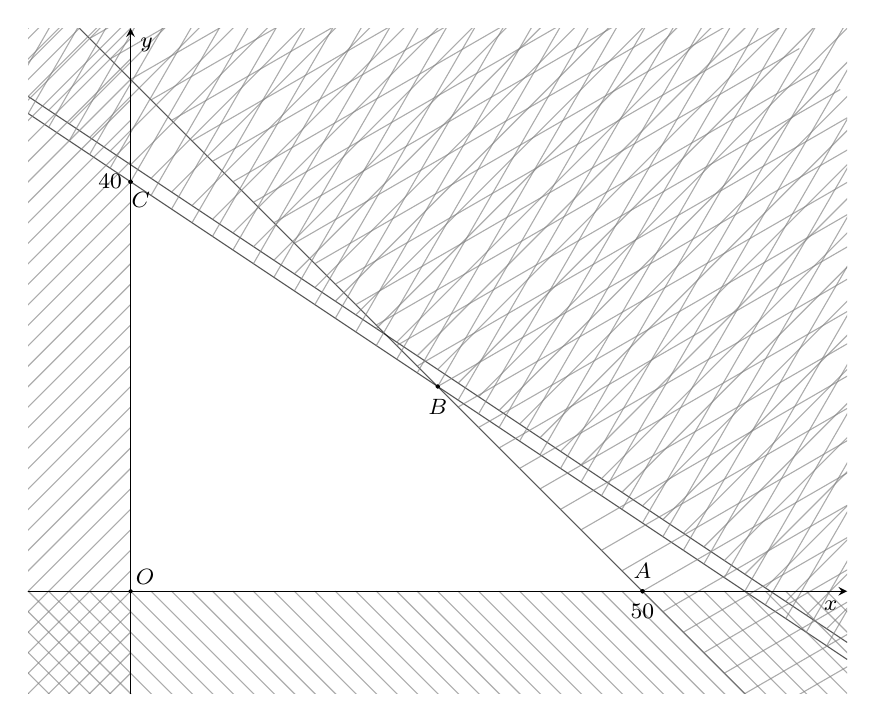
\begin{tikzpicture}[font=\footnotesize, line join=round, line cap=round, >=stealth,xscale=.13,yscale=.13]
			\def\fx{(-2/3)*(\x)+125/3}
			\def\gx{(-2/3)*(\x)+40}
			\def\hx{-(\x)+50}
			\begin{scope}[opacity=.65]
				\clip (-10,-10)rectangle(70,55);
				\draw[samples=100,domain=-20:70]plot(\x,{\fx});
				\draw[samples=100,domain=-20:70]plot(\x,{\gx});
				\draw[samples=100,domain=-20:70]plot(\x,{\hx});
				
				\foreach \i in{-20,-18,...,68,70}{
				\def\x{\i}
				\draw[gray](\x,{\fx})--++(45:60);
				\draw[gray](\x,{\gx})--++(60:60);
				\draw[gray](\x,{\hx})--++(30:50);
				\draw[gray](\x,0)--++(-45:60);
				\draw[gray](0,\i)--++(-135:60);
				}
			\end{scope}
			\draw[->](-10,0)--(70,0)node[below left]{$x$};
			\draw[->](0,-10)--(0,55)node[below right]{$y$};
			\foreach \x/\y/\m/\g in{0/0/O/45,0/40/40/-180,0/40/C/-60,50/0/50/-90,50/0/A/90,30/20/B/-90}
			\draw[fill=black](\x,\y)circle(5pt)++(\g:2)node{$\m$};
		\end{tikzpicture}
	\end{center}
	Hàm số $F(x;y)=5x+7y$ sẽ đạt giá trị lớn nhất trên miền nghiệm của hệ bất phương trình khi $(x;y)$ là tọa độ một trong các đỉnh $O(0;0)$, $A(50;0)$, $B(30;20)$, $C(0;40)$.\\
	Mà $F(0;0)=0$; $F(50; 0)=250$; $F(30;20)=290$; $F(0;40)=280$.\\
	Suy ra $F(x;y)$ lớn nhất khi $(x;y)=(30;20)$.\\
	Vậy cần gói $30$ cái bánh chưng và $20$ cái bánh ống để đạt được số điểm thưởng cao nhất nên $a=30$, $b=20$. Suy ra $b-a=-10$.
	}
\end{ex}

\begin{ex}%[0D8V2-6]
	Cho đa giác đều $(H)$ có $15$ đỉnh. Người ta lập một tứ giác có $4$ đỉnh là $4$ đỉnh của $(H)$. Tính số tứ giác được lập thành mà không có cạnh nào là cạnh của $(H)$.
	\shortans[oly]{$450$}
	\loigiai{
	Gọi đa giác là $A_1A_2\ldots A_{15}$. Giả sử chọn đỉnh thứ nhất là $A_1$.\\
	Ta chọn các đỉnh còn lại theo thứ tự tứ giác là $A_m$,  $A_n$,  $A_p$.\\
	Gọi số đỉnh nằm giữa $A_1$ và $A_m$ là $x$; số đỉnh nằm giữa $A_m$ và $A_n$ là $y$; số đỉnh nằm giữa $A_n$ và $A_p$ là $z$; số đỉnh nằm giữa $A_p$ và $A_1$ là $t$. Khi đó, ta có hệ
	\[\heva{&x+y+z+t=11\\&x,y,z,t\ge 1\\&x,y,z,t\in \mathbb{N}.}\quad (1)\]
	Xếp $11$ thước kẻ nhỏ thành một hàng ngang suy ra có $10$ khoảng trống giữa các thước này. Số nghiệm của hệ $(1)$ là số cách đặt $3$ thước kẻ lớn vào $10$ khoảng trống kia để chia làm bốn phần: có $\mathrm{C}^3_{10}$ cách đặt.\\
	Do đó, hệ $(1)$ có $\mathrm{C}^3_{10}$ nghiệm.\\
	Như vậy có $15\cdot\mathrm{C}^3_{10} $ tứ giác thỏa mãn.\\
	Tuy nhiên, theo cách chọn này,	mỗi tứ giác $A_1A_mA_nA_p$ lặp lại $4$ lần khi chọn các đỉnh thứ nhất lần lượt là $A_1$, $A_m$, $A_n$, $A_p$.\\
	Do đó, số tứ giác cần tính là $\dfrac{15\cdot\mathrm{C}^3_{10}}{4}=450$.
	}
\end{ex}

\begin{ex}%[2D4V3-3]
	Một quả trứng khủng long đồ chơi bằng nhựa có thiết diện qua trục lớn là một đường elip. Biết độ dài mỗi trục là $12$ cm và $8$ cm.
	Bên trong quả trứng người ta cần thiết kế một chiếc hộp hình trụ để đựng các đồ chơi trẻ con như bóng đèn xanh đỏ, kẹo $\ldots$
	Hỏi khối trụ như thế có thể tích tối đa bao nhiêu cm$^3$ (làm tròn đến hàng đơn vị)?
	\begin{center}
		\begin{tikzpicture}[line join=round, line cap=round,>=stealth,font=\footnotesize,scale=0.9]
			\path (0,0) coordinate (O);
			\draw (O) ellipse (3 cm and 2 cm);
			\path ($(O) + (40:3 and 2)$) coordinate (A)
			($(O) + (140:3 and 2)$) coordinate (B)
			($(O) + (220:3 and 2)$) coordinate (C)
			($(O) + (-40:3 and 2)$) coordinate (D)			;
			\draw[dashed] (A)--(B) (C)--(D)
			(A) to [bend right=20](D)
			(B) to [bend right=20](C)
			;
			\draw (A) to [bend left=20](D)
			(B) to [bend left=20](C)
			;
			\foreach \t/\g in {A/90,B/90,C/180,D/0}{
			\draw[fill=black] (\t) circle (1pt) ;
			}
		\end{tikzpicture}
	\end{center}
	\shortans{232}
	\loigiai{
	\begin{center}
		\begin{tikzpicture}[line join=round, line cap=round,>=stealth,font=\footnotesize,scale=0.9]
			\path (0,0) coordinate (O);
			\draw (O) ellipse (3 cm and 2 cm);
			\path ($(O) + (40:3 and 2)$) coordinate (A)
			($(O) + (140:3 and 2)$) coordinate (B)
			($(O) + (220:3 and 2)$) coordinate (C)
			($(O) + (-40:3 and 2)$) coordinate (D)	;
			\draw[->] (-4,0)--(4,0)node[below]{$x$};
			\draw[->] (0,-3)--(0,3)node[left]{$y$};
			\draw[dashed] (A)--(B) (C)--(D)
			(A) to [bend right=20](D)
			(B) to [bend right=20](C)
			;
			\draw (A) to [bend left=20](D)
			(B) to [bend left=20](C)
			;
			\foreach \t/\g in {A/90,B/90,C/180,D/0}{
			\draw[fill=black] (\t) circle (1pt);
			}
			\foreach \t/\g in {O/230,A/90}{
			\draw[fill=black] (\t) circle (1pt) node[shift={(\g:7pt)},font=\scriptsize]{$ \t $};
			}
		\end{tikzpicture}
	\end{center}
	Gắn elip lên hệ trục tọa độ $Oxy$ như hình vẽ, elip có \[2a=12\Rightarrow a=6; 2b=8\Rightarrow b=4.\]
	Phương trình chính tắc elip $(E)\colon\dfrac{x^2}{36}+\dfrac{y^2}{16}=1$.\\
	Đặt chiều cao và bán kính đáy hình trụ nội tiếp elip là $h$, $r$ thì điểm tiếp xúc $A\left(\dfrac{h}{2}; r\right)$ với $0< h < 12$; $0< r < 4$.\\
	Điểm $A$ thuộc $(E)\colon\dfrac{x^2}{36}+\dfrac{y^2}{16}=1\Rightarrow \dfrac{\left(\dfrac{h}{2} \right)^2}{36}+\dfrac{r^2}{16}=1
	\Rightarrow \dfrac{h^2}{144}+\dfrac{r^2}{16}=1\Rightarrow r^2=16\left(1-\dfrac{h^2}{144}\right)$.\\
	Thể tích khối trụ là $V=\pi r^2h=\pi \cdot16\left(1-\dfrac{h^2}{144} \right)\cdot h=\pi \left(16h-\dfrac{h^3}{9} \right)$.\\
	Ta có $V'=\pi \left(16-\dfrac{h^2}{3} \right)$;
	$V'=0\Rightarrow 16-\dfrac{h^2}{3}=0\Rightarrow h^2=48\Rightarrow h=4\sqrt{3} \in (0; 12)$.\\
	Bảng biến thiên
	\begin{center}
		\begin{tikzpicture}[font=\normalsize,t style/.style={style=solid}]
			\tkzTabInit[nocadre=false, lgt=1.2, espcl=2.5, deltacl=0.5]%,help]
			{$h$/0.7, $V'$/0.7, $V$/2}
			{$0$, $4\sqrt{3}$, $12$}
			\tkzTabLine{ , +, 0, -}
			\path
			($(N13)!0.1!(N12)$) node (A1){}
			($(N23)!0.8!(N22)$) node (A2){}
			($(N33)!0.1!(N32)$) node (A3){};
			\foreach \x/\y in {A1/A2, A2/A3}{
			\draw[-stealth] (\x)--(\y);
			}
		\end{tikzpicture}
	\end{center}
	Giá trị lớn nhất của thể tích khối trụ là \[V_{\max}=V\left(4\sqrt{3} \right)=\pi \left(16\cdot 4\sqrt{3}-\dfrac{\left(4\sqrt{3} \right)^3}{9} \right)\approx 232\ (\mathrm{cm}^3).\]
	}
\end{ex}
\Closesolutionfile{ans}
% \indapan{6}{ans/2-PT-TNTHPT2025-De1-KQ}
